\documentclass[12pt,twoside]{article}
\usepackage[dvipsnames]{xcolor}
\usepackage{tikz,graphicx,amsmath,amsfonts,amscd,amssymb,bm,cite,epsfig,epsf,url}
\usepackage[hang,flushmargin]{footmisc}
\usepackage[colorlinks=true,urlcolor=blue,citecolor=blue]{hyperref}
\usepackage{amsthm,multirow,wasysym,appendix}
\usepackage{array,subcaption} 
% \usepackage[small,bf]{caption}
\usepackage{bbm}
\usepackage{pgfplots}
\usetikzlibrary{spy}
\usepgfplotslibrary{external}
\usepgfplotslibrary{fillbetween}
\usetikzlibrary{arrows,automata}
\usepackage{thmtools}
\usepackage{blkarray} 
\usepackage{textcomp}
\usepackage[left=0.8in,right=1.0in,top=1.0in,bottom=1.0in]{geometry}
\usepackage{pdfpages}
\newcommand*{\defeq}{\stackrel{\text{def}}{=}}
\newcommand{\R}{\mathbb{R}}
\newcommand{\rank}{rank}
\newcommand{\Tr}{Trace}
\title{Linear Algebra HW 8}
\author{gjd9961 }
\date{November 2021}

\begin{document}

\maketitle


\section{Problem 8.1}
	Let $A \in \R^{n \times m}$. The Singular Values Decomposition (SVD) tells us that there exists two orthogonal matrices $U \in \R^{n \times n}$ and $V \in \R^{m \times m}$ and a matrix $\Sigma \in \R^{n \times m}$ such that $\Sigma_{1,1} \geq \Sigma_{2,2}  \geq \cdots \geq 0$ and $\Sigma_{i,j} = 0$ for $i\neq j$
	$$
	A = U \Sigma V^{\sT}.
	$$
	The columns $u_1, \dots, u_n$ of $U$ (respectively the columns $v_1, \dots, v_m$ of $V$) are called the left (resp.\ right) singular vectors of $A$. The non-negative numbers $\sigma_i \defeq \Sigma_{i,i}$ are the singular values of $A$. Moreover we also know that $$r \defeq \rank(A) = \# \{i \, | \, \Sigma_{i,i} \neq 0 \}$$
	
a) Let 
			$\widetilde{U} = \!
			{\small \begin{pmatrix}
					| & & | \\
					u_1 & \!\cdots\! & u_r \\
					| & & | 
			\end{pmatrix} } \! \in \! \R^{n \times r}$ ,
			$\widetilde{V} = \!
			{\small \begin{pmatrix}
					| & & | \\
					v_1 & \!\cdots\! & v_r \\
					| & & | 
			\end{pmatrix} } \! \in \! \R^{m \times r}$ and
			$\widetilde{\Sigma} = \Diag(\sigma_1, \dots, \sigma_r) \in \R^{r \times r}$.\\
			Show that $A = \widetilde{U}\widetilde{\Sigma}\widetilde{V}^T$.\\
			
Let $x$ be a vector in the input space, $x\in \R^m$ and $x$ be some linear combination of the orthonormal vectors of $V$, $x=\alpha_1v_1 + \dots + \alpha_m v_m$. Let $y$ be a vector in the output space, $\R^n$, such that $Ax=y$ and therefore $U\Sigma V^Tx = y$. Therefore, $y\in Im(A)$ and $y\in Im(U\Sigma V^Tx)$. Let $r=Rank(A)$.
Lets approach the problem one step at a time. What does $V^Tx$ equal?
\begin{equation}
    \begin{split}
        V^Tx = \begin{pmatrix}
					-- & v_1 & -- \\
					-- & \dots & -- \\
					-- & v_m & --  
			\end{pmatrix}\begin{pmatrix}
			| \\
					x \\
					|
			\end{pmatrix} = \begin{pmatrix}
			\alpha_1 \\
			| \\
			\alpha_m
			\end{pmatrix}
    \end{split}
\end{equation}
This is because matrix vector multiplication is the dot product of the rows of the matrix and the vector column, and since the vector $x$ is a linear combination of the orthonormal columns of V we have:
$$
    \langle v_i, x \rangle = \langle v_i, \alpha_1 v_1 + \dots + v_m\alpha_m \rangle = \langle v_i, v_1\alpha_1 \rangle + \dots + \langle v_i, v_m\alpha_m \rangle $$
Where we have for any $\langle v_i, \alpha_jv_j \rangle = \alpha_j$ if $v_i=v_j$, otherwise if $v_i \neq v_j$ then we have $\langle v_i, \alpha_jv_j \rangle =0$
Now that we know what $V^Tx$ is, lets figure out what $\Sigma V^Tx$ is. Remember, $\Sigma$ is a $\R^{n\times m}$ matrix, whose diagonals are the singular values of the matrix $A$ and that $r$ of them will be non zero.
$$
    \Sigma V^Tx = \begin{pmatrix}
    \sigma_{1,1} & \dots & \dots & \dots & 0_{1,m}\\
    0 & \sigma_{2,2} & \dots & \dots & 0 \\
    \vdots & & \ddots & \sigma_{r,r} & 0\\
    0_{n,1} & \dots & \dots & \dots & 0_{n,m}
    \end{pmatrix} \begin{pmatrix}
			\alpha_1 \\
			| \\
			\alpha_m
			\end{pmatrix} = 
			\begin{pmatrix}
			\alpha_1 \times \sigma_1 \\
			\vdots \\
			\alpha_r \times \sigma_r \\
			0 \\
			\vdots \\
			0
			\end{pmatrix}
$$
So the resulting output vector of $\Sigma V^T x$ will be a vector with its first $r$ entries equal to $\alpha_i\times \sigma_i$ for $i \in \{1,\dots, r\}$ and the rest of the values (values $r+1$ through $n$) will be equal to 0.
Lastly, lets see what happens when we do the whole thing: $U\Sigma V^T x$
$$
U\Sigma V^T x = 
    \begin{pmatrix}
					| & & | \\
					u_1 & \!\cdots\! & u_n \\
					| & & | 
			\end{pmatrix}\begin{pmatrix}
			\alpha_1 \times \sigma_1 \\
			\vdots \\
			\alpha_r \times \sigma_r \\
			0 \\
			\vdots \\
			0
			\end{pmatrix} = \sum_{i=1}^r \alpha_i \times \sigma_i \times u_i + \sum_{j=r+1}^n 0 \times u_j = \sum_{i=1}^r \alpha_i \times \sigma_i \times u_i = y
$$
The process is the same for $\widetilde{U}\widetilde{\Sigma}\widetilde{V}^Tx$, 
Therefore:

\begin{equation}
    \begin{split}
        Ax &= Ax \\
        U\Sigma V^Tx &= \widetilde{U}\widetilde{\Sigma}\widetilde{V}^Tx\\
        \sum_{i=1}^r \alpha_i \times \sigma_i \times u_i + \sum_{j=r+1}^n 0 \times u_j &= \sum_{i=1}^r \alpha_i \times \sigma_i \times u_i\\
        \sum_{i=1}^r \alpha_i \times \sigma_i \times u_i &= \sum_{i=1}^r \alpha_i \times \sigma_i \times u_i
    \end{split}
\end{equation}

That shows the equivalence for matrix vector multiplication, but we can show this without needing the vector. In general, any entry $i,j$ in the matrix product of $U\Sigma V^T$ is equal to the entry in the matrix product of  $\widetilde{U}\widetilde{\Sigma}\widetilde{V}^T$. We can show this as follows: 

\begin{equation}
    \begin{split}
        (U\Sigma V^T)_{i,j}  &= (\widetilde{U}\widetilde{\Sigma}\widetilde{V}^T)_{i,j} \\
        \sum_{l=1}^n  u_{i,l} \times \sigma_{i} \times v_{l,j}^T  &=  \sum_{l=1}^r  u_{i,l} \times \sigma_{i} \times v_{l,j}^T \\
        \sum_{l=1}^r  u_{i,l} \times \sigma_{i} \times v_{l,j}^T + \sum_{l=r+1}^n 0 \times u_j &=  \sum_{l=1}^r  u_{i,l} \times \sigma_{i} \times v_{l,j}^T \\
        \sum_{l=1}^r  u_{i,l} \times \sigma_{i} \times v_{l,j}^T &= \sum_{l=1}^r  u_{i,l} \times \sigma_{i} \times v_{l,j}^T \qed
    \end{split}
\end{equation}

This further proves their equivalence. 






	\newpage
	
b) Give orthonormal bases of $Ker(A)$ and $Im(A)$ in terms of the singular vectors $u_1, \dots, u_n$ and $v_1, \dots , v_m$. \\

Firstly for the basis of Im(A). Let $x$ be a vector in the input space, $x\in \R^m$ and $x$ be some linear combination of the orthonormal vectors of $V$, $x=\alpha_1v_1 + \dots + \alpha_m v_m$. Let $y$ be a vector in the output space, $\R^n$, such that $Ax=y$ and therefore $U\Sigma V^Tx = y$. Therefore, $y\in Im(A)$ and $y\in Im(U\Sigma V^Tx)$. Let $r=Rank(A)$.

Lets approach the problem one step at a time. What does $V^Tx$ equal?
\begin{equation}
    \begin{split}
        V^Tx = \begin{pmatrix}
					-- & v_1 & -- \\
					-- & \dots & -- \\
					-- & v_m & --  
			\end{pmatrix}\begin{pmatrix}
			| \\
					x \\
					|
			\end{pmatrix} = \begin{pmatrix}
			\alpha_1 \\
			| \\
			\alpha_m
			\end{pmatrix}
    \end{split}
\end{equation}
This is because matrix vector multiplication is the dot product of the rows of the matrix and the vector column, and since the vector $x$ is a linear combination of the orthonormal columns of V we have:
$$
    \langle v_i, x \rangle = \langle v_i, \alpha_1 v_1 + \dots + v_m\alpha_m \rangle = \langle v_i, v_1\alpha_1 \rangle + \dots + \langle v_i, v_m\alpha_m \rangle $$
Where we have for any $\langle v_i, \alpha_jv_j \rangle = \alpha_j$ if $v_i=v_j$, otherwise if $v_i \neq v_j$ then we have $\langle v_i, \alpha_jv_j \rangle =0$
Now that we know what $V^Tx$ is, lets figure out what $\Sigma V^Tx$ is. Remember, $\Sigma$ is a $\R^{n\times m}$ matrix, whose diagonals are the singular values of the matrix $A$ and that $r$ of them will be non zero.
$$
    \Sigma V^Tx = \begin{pmatrix}
    \sigma_{1,1} & \dots & \dots & \dots & 0_{1,m}\\
    0 & \sigma_{2,2} & \dots & \dots & 0 \\
    \vdots & & \ddots & \sigma_{r,r} & 0\\
    0_{n,1} & \dots & \dots & \dots & 0_{n,m}
    \end{pmatrix} \begin{pmatrix}
			\alpha_1 \\
			| \\
			\alpha_m
			\end{pmatrix} = 
			\begin{pmatrix}
			\alpha_1 \times \sigma_1 \\
			\vdots \\
			\alpha_r \times \sigma_r \\
			0 \\
			\vdots \\
			0
			\end{pmatrix}
$$
So the resulting output vector of $\Sigma V^T x$ will be a vector with its first $r$ entries equal to $\alpha_i\times \sigma_i$ for $i \in \{1,\dots, r\}$ and the rest of the values (values $r+1$ through $n$) will be equal to 0.
Lastly, lets see what happens when we do the whole thing: $U\Sigma V^T x$
$$
U\Sigma V^T x = 
    \begin{pmatrix}
					| & & | \\
					u_1 & \!\cdots\! & u_n \\
					| & & | 
			\end{pmatrix}\begin{pmatrix}
			\alpha_1 \times \sigma_1 \\
			\vdots \\
			\alpha_r \times \sigma_r \\
			0 \\
			\vdots \\
			0
			\end{pmatrix} = \sum_{i=1}^r \alpha_i \times \sigma_i \times u_i + \sum_{j=r+1}^n 0 \times u_j = \sum_{i=1}^r \alpha_i \times \sigma_i \times u_i = y
$$
To recap what we have shown is that $y\in Im(A)$ is a linear combination of the first $r$ columns of the orthonormal matrix $U$. That is to say:
\begin{equation}
    \begin{split}
        y &= Ax \qquad \text{By definition} \\
        y &= U\Sigma V^Tx  \qquad \text{By SVD} \\
        y &= \sum_{i=1}^r \sigma_i \times \alpha_i \times u_i \qed
    \end{split}
\end{equation}
Therefore, the basis of Im(A) can be expressed by the orthonormal basis $\{u_1, \dots, u_r\}$\\

Now we can repeat this exact process, but we need to add an additional assumption. Let $r=Rank(A)$ and $r < m < n $, such that $dim(Ker(A)) \geq 1$. Let $x\in \R^m$ and $x\in Ker(A)$ such that $Ax = 0$ and $U\Sigma V^T x = 0$. Let $\alpha_1, \dots, \alpha_m \in \R$ and $x$ be the linear combination of $x= \alpha_1 v_1 + \dots + \alpha_m v_m$ where $\alpha_i=0$ for $\alpha_1 \dots \alpha_r$ and $\alpha_i$ non zero for $\alpha_{r+1}, \dots, \alpha_m$

Lets approach the problem one step at a time. What does $V^Tx$ equal?
\begin{equation}
    \begin{split}
        V^Tx = \begin{pmatrix}
					-- & v_1 & -- \\
					-- & \dots & -- \\
					-- & v_m & --  
			\end{pmatrix}\begin{pmatrix}
			| \\
					x \\
					|
			\end{pmatrix} = \begin{pmatrix}
			0 \\
			| \\
			\alpha_{r+1} \\
			| \\
			\alpha_m
			\end{pmatrix}
    \end{split}
\end{equation}
This is because matrix vector multiplication is the dot product of the rows of the matrix and the vector column, and since the vector $x$ is a linear combination of the orthonormal columns of V we have:
$$
    \langle v_i, x \rangle = \langle v_i, \alpha_1 v_1 + \dots v_m\alpha_m \rangle = \langle v_i, v_1\alpha_1 \rangle + \dots + \langle v_i, v_m\alpha_m \rangle $$
Where we have for any $\langle v_i, \alpha_jv_j \rangle = \alpha_j$ if $v_i=v_j$, otherwise if $v_i \neq v_j$ then we have $\langle v_i, \alpha_jv_j \rangle =0$\\

In other words, the first $r$ entries of $V^Tx$ are equal to 0, and the entries from $r+1$ to $m$ are equal to their respective $\alpha$ values. Now that we know what $V^Tx$ is, lets figure out what $\Sigma V^Tx$ is.\\

Remember, $\Sigma$ is a $\R^{n\times m}$ matrix, whose diagonals are the singular values of the matrix $A$ and that $r$ of them will be non zero.
$$
    \Sigma V^Tx = \begin{pmatrix}
    \sigma_{1,1} & \dots & \dots & \dots & 0_{1,m}\\
    0 & \sigma_{2,2} & \dots & \dots & 0 \\
    \vdots & & \ddots & \sigma_{r,r} & 0\\
    0_{n,1} & \dots & \dots & \dots & 0_{n,m}
    \end{pmatrix} \begin{pmatrix}
			0 \\
			\vdots \\
			\alpha_{r+1} \\
			\vdots \\
			\alpha_m
			\end{pmatrix} = \sum_{i=1}^r \sigma_i \times 0 + \sum_{j=r+1}^m 0 \times \alpha_j = 
			\begin{pmatrix}
			0 \\
			\vdots \\
			0
			\end{pmatrix}
$$
So the resulting output vector of $\Sigma V^T x$ will be a vector with all of its entries equal to 0. \\
.
Lastly, lets see what happens when we do the whole thing: $U\Sigma V^T x$
$$
U\Sigma V^T x = 
    \begin{pmatrix}
					| & & | \\
					u_1 & \!\cdots\! & u_n \\
					| & & | 
			\end{pmatrix} \begin{pmatrix}
			0 \\
			\vdots \\
            0
			\end{pmatrix} = \sum_{i=1}^n 0 \times u_i = 0
			$$
To recap what we have shown is that $x\in Ker(A)$ is a linear combination of the $r+1$ through $m$ columns of the orthogonal matrix $V$. Therefore, the basis for Ker(A) can be expressed by the orthonormal basis $\{v_{r+1}, \dots, v_m\}$\\

















\vspace{5mm}

\section{Problem 8.2}
	For any two matrices $A,B \in \R^{n\times m}$ we define the \emph{Frobenius inner-product} as
	$$
	\langle A,B \rangle_{F} = \Tr(A^{\sT} B).
	$$
	We showed in the midterm that it verifies the points of the definition~2.1 of Lecture~4 for the square matrix case (one can also check that it works for rectangular matrices). Show that the induced norm $\|A\|_F = \sqrt{\Tr(A^T A)}$ can be computed as a function of the singular values $\sigma_1, \dots, \sigma_{\min(n,m)}$ of $A$ as
			$$
			\|A\|_F = \sqrt{\sum_{i=1}^{\min(n,m)} \sigma_i^2}
			.$$
To answer this question, we will need to use a fact we proved in past home-works: that $Trace(BC) = Trace(CB)$.  Let the SVD of A equal $A=U\Sigma V^T$ where U and V are orthogonal matrices in $\R^{n\times n}$ and $\R^{m \times m}$ respectively, and $\Sigma$ be the diagonal matrix of singular values $\sigma_1, \dots, \sigma_{\min(n,m)}$ of $A$. Also, let B,C be two rectangular matrices, such that $B=V\Sigma^T$ and $C=\Sigma V^T$.
\begin{equation}
    \begin{split}
        \langle A,A\rangle &= \sqrt{Trace(A^TA)} \text{ By definition of Problem Statement} \\
        \langle A,A\rangle &= \sqrt{Trace((U\Sigma V^T)^T(U\Sigma V^T))} \text{ By SVD} \\
        \langle A,A\rangle &= \sqrt{Trace(V\Sigma^TU^T U\Sigma V^T)} \text{ Distribute Transpose} \\
        \langle A,A\rangle &= \sqrt{Trace(V\Sigma^T\Sigma V^T)} \text{ as } U^TU = Id_n \\
        \langle A,A\rangle &= \sqrt{Trace(BC)} \text{ Substitute Identities }   \\
        \langle A,A\rangle &= \sqrt{Trace(CB)} \text{ using } Trace(BC)=Trace(CB)    \\
        \langle A,A\rangle &= \sqrt{Trace(\Sigma V^TV\Sigma^T)} \text{ Substitute Identities } \\
        \langle A,A\rangle &= \sqrt{Trace(\Sigma\Sigma^T)} \text{ as } V^TV = Id_n\\
        \langle A,A\rangle &= \sqrt{\sum_{i=1}^{\min(n,m)} \sigma_i^2} \\
        \|A\|_F &= \sqrt{\sum_{i=1}^{\min(n,m)} \sigma_i^2} \qed
    \end{split}
\end{equation}


\vspace{1mm}

\newpage 


\section{Problem 8.3}

a) Show that $\mathcal{H}(1)$ is true.\\

$\mathcal{H}(1)$ is true by the definition of the adjacency matrix of graph G.  Taking $k=1$ we want to prove that $A^1$ represents the number of ways to go from $i$ to $j$ in a single step. And, it just so happens, by definition, the adjacency matrix's entries of $A_{i,j}$ describe the number of ways to go from $i$ to $j$ in one step, therefore it holds true for when $k=1$. We can illustrate this in the following way. Consider a the following graph and its related adjacency matrix:\\


\begin{figure}[h!]
    \centering
    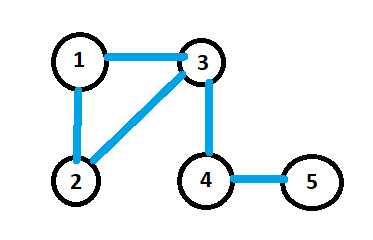
\includegraphics[scale=1]{graph for 8.3.png}
    \caption{Graph G}
    \label{fig:my_label}
\end{figure}

Its adjacency matrix, $A_{i,j}^1=A_{i,j}$ is the number of ways we can go from $i$ to $j$ (or vica versa if we look at $A_{j,i}$ as the adjacency matrix is symmetric) in 1 step.

$$
    Adjacency \ Matrix \ of \ G = A = 
    \begin{pmatrix} 
    0 & 1 & 1 & 0 & 0 \\
    1 & 0 & 1 & 0 & 0 \\
    1 & 1 & 0 & 1 & 0 \\
    0 & 0 & 1 & 0 & 1 \\
    0 & 0 & 0 & 1 & 0 
    \end{pmatrix}
$$
\\

b) Show that if $\mathcal{H}(k)$ is true for some $k$, then $\mathcal{H}(k+1)$ is also true.\\

Knowing what we know if part 1, that $\mathcal{H}(1)$ holds, we can show that $\mathcal{H}(1+1) = \mathcal{H}(2)$ is equal to $A^1 \times A^{k-1}$ where $A$ is the adjacency matrix, and $k=2$, and that $A_{i,j}^2$ represents the amount of paths of $i$ to $j$ with length 2. As all adjacency matrices are square symmetric, proving any arbitrary example will hold for all adjacency matrices. We will demonstrate with our graph $G$ and our adjacency matrix $A$, and then generalize our solution to all adjacency matrices.

$$
    A^{k-1} \times A = \begin{pmatrix} 
    2 & 1 & 1 & 1 & 0 \\
    1 & 2 & 1 & 1 & 0 \\
    1 & 1 & 3 & 0 & 1 \\
    1 & 1 & 0 & 2 & 0 \\
    0 & 0 & 1 & 0 & 1 
    \end{pmatrix}
$$
Consulting with the graph in Figure 1, we can see that $A_{i,j}^2$ accurately describes all the paths from $i$ to $j$ in length $k$ $(2)$ steps. Since we have shown how $\mathcal{H}(k)$ where k=1 and $\mathcal{H}(k+1)$ where $k+1 = 2$ holds, we can generalize our solution for any positive integer $k$. \\

We have shown that our solution works for our base case, $\mathcal{H}(k)$ where $k=1$, and that it works for any $\mathcal{H}(k+1)$ where $k$ is a positive integer, then we know that any $\mathcal{H}(k)$ can be expressed as $\mathcal{H}(k)=A^k$, it follows that it can be expressed as $A^k_{ij} = \sum\limits^n_{l=1}A^{k-1}_{il}*A_{lj}$ where $A^{k-1}_{il}$ represents the number of ways to get from $i$ to $l$ in $k-1$ steps and $A_{lj}$ is the number of ways to get from $l$ to $i$ in 1 step. We can do this for any positive integer $k$ and it will hold. Therefore:

$$A^{k+1}_{ij} = \sum\limits^n_{l=1}A^{k}_{il}*A_{lj} \qed $$


\vspace{1mm}


\section{Problem 8.4}
	The goal of this problem is to use spectral clustering techniques on real data.
	The file \texttt{adjacency.txt} contains the adjacency matrix of a graph taken from a social network. This graphs has $n=328$ nodes (that corresponds to users). An edge between user $i$ and user $j$ means that $i$ and $j$ are ``friends'' in the social network.
	The notebook \texttt{friends.ipynb} contains functions to read the adjacency matrix as well as instructions/questions.
	\\

	While we focused in the lectures (and in the notes) on the graph Laplacian
	$$
	L = D - A,
	$$
	where $A$ is the adjacency matrix of the graph, and $D = \Diag(\deg(1), \dots, \deg(n))$ is the degree matrix, we will use here the ``normalized Laplacian'' (instead of $L$)
	$$
	L_{\rm norm} = D^{-1/2} L D^{-1/2} = \Id_n - D^{-1/2} A D^{-1/2},
	$$
	where $D^{-1/2} = \Diag(\deg(1)^{-1/2}, \dots, \deg(n)^{-1/2})$. The reason for using a different Laplacian is that then ``unnormalized Laplacian'' $L$ does not perform well when the degrees in the graph are very broadly distributed, i.e. very heterogeneous. In such situations, the normalized Laplacian $L_{\rm norm}$ is supposed to lead to a more consistent clustering.

	\textbf{It is intended that you code in Python and use the provided Jupyter Notebook. Please only submit a pdf version of your notebook (right-click $\to$ `print' $\to$ `Save as pdf').}

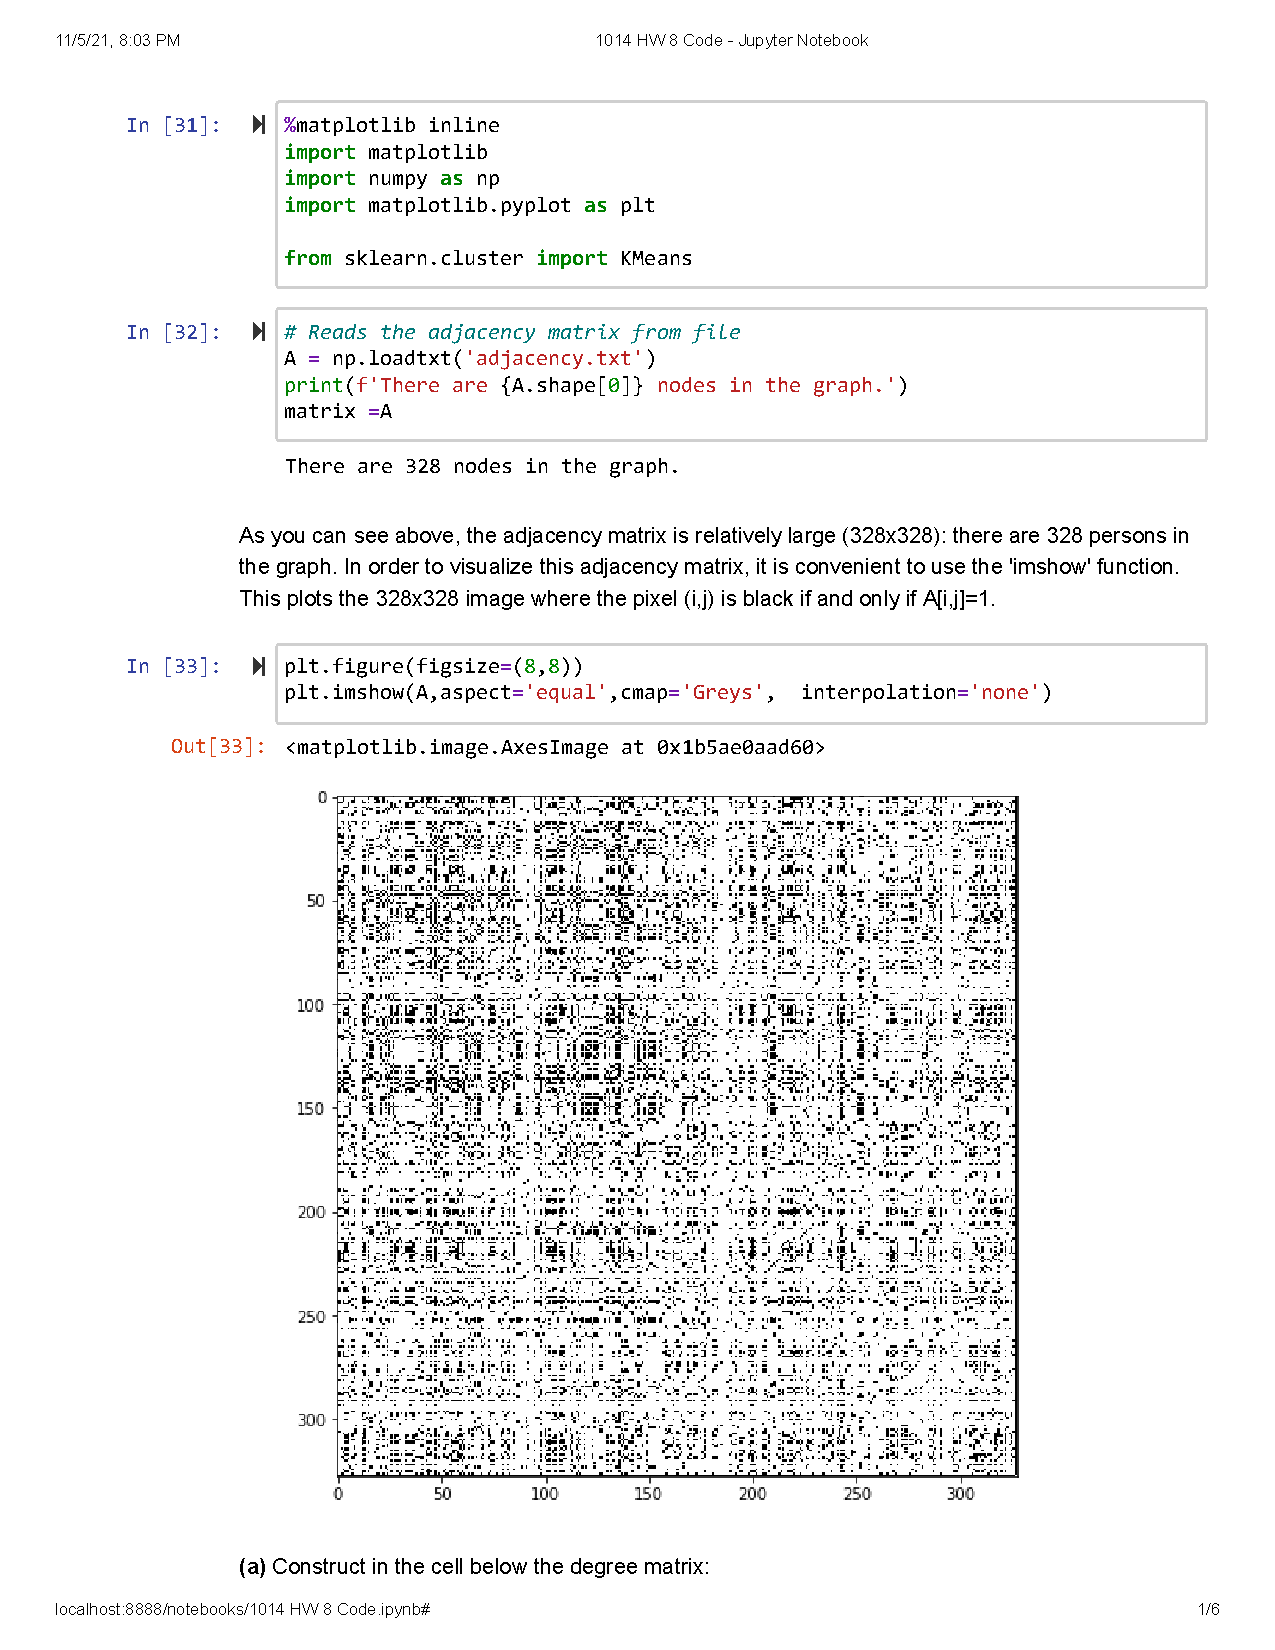
\includepdf[pages=-]{1014 hw 6 code.pdf}

\vspace{5mm}

\section{Problem 8.5 (Extra Credit)}
	Let $G$ be a connected graph with $n$ nodes. Define $L \in \R^{n \times n}$ the associate Laplacian matrix and $\lambda_1 \leq \lambda_2 \leq \cdots \leq \lambda_n$ its eigenvalues. Let $G'$ be a graph constructed from $G$ by simply adding an edge. Similarly denote by $\lambda_2'$ its second smallest eigenvalue. Show that  $\lambda_2' \geq \lambda_2$. \\

 

In general, if we add an edge connecting two nodes, $i$ and $j$, in Graph G, (meaning we connect nodes $i$ and $j$ to each other with a single edge), the corresponding entries of the associated Laplacian matrix, $L$, will decrease by 1 at $L_{ij},  L_{ji},$ and increase at $L_{ii}$ and $L_{jj}$ by one, as the entries are connected and the Lapliacian is defined as $L=D-A$ where $D$ is the Degree matrix and $A$ is the Adjacency matrix of Graph $G'$. We call the Laplacian matrix of graph $G'$, $L'$. \\

We know from past homeworks that for any square symmetric matrices $A\in \R^{n \times n}$ that the $Trace(A)$ is equal to the sum of its eigenvalues. That is to say: $Trace(A) = Trade(D)$ where $D$ is the diagonal matrix of $A's$ eigenvalues. When we added an edge, we increased the entries of the diagonals, that is to say $Trace(L') > Trace(L)$ and since $L$ and $L'$ are square symmetric matrices, it follows that $Trace(Eigenvalues \ of \ L') > Trace(Eigenvalues \ of \ L)$. \\

Furthermore, we know that $\lambda_2' \geq \lambda_2$ as when we add an edge it increases the graph's overall connectivity and in turn increase the graph's algebraic connectivity value of ($\lambda_2$). If we successfully added an edge between two unconnected nodes, it follows that $\lambda_2' > \lambda_2$, and in the case that the graph G is already fully connected, adding an edge does not increase connectivity thus its algebraic connectivity value remains the same, which would mean $\lambda_2' = \lambda_2$. So in general, when adding an edge to a graph, it follows that $\lambda_2' \geq \lambda_2$.
\end{document}
